% !TEX encoding   = UTF8
% !TEX spellcheck = ru_RU

\documentclass[a4paper,11pt,landscape,notitlepage,oneside,openany,final]{memoir}

% !TEX encoding   = UTF8
% !TEX spellcheck = en_US


%%% Page layout %%%
\usepackage{pdflscape}
\usepackage{geometry}

%%% Mathematics %%%
\usepackage{amsthm,amsfonts,amsmath,amscd}
\usepackage{mathtools}             % Add environment 'multlined'
\usepackage{dsfont}
\usepackage{unicode-math}

%%% Encodings and fonts %%%
\usepackage{polyglossia}[2014/05/21]  % Automatically load 'fontspec'

%%% Paragraph layout %%%
\usepackage{indentfirst}
\usepackage{epigraph}
\usepackage[style=french]{csquotes}

%%% Colors %%%
\usepackage[svgnames,table,hyperref]{xcolor} %,cmyk

%%% Tables %%%
\usepackage{longtable,ltcaption}
\usepackage{multirow,makecell}     % Advanced formatting
\usepackage{tabu,tabulary}         % Automatic columns width
\usepackage{array}
\usepackage{hhline}
\usepackage{multicol}

%%% General layout %%%
\usepackage{soulutf8}              % Underlying with hyphenation
\usepackage{icomma}
\usepackage{calc}
\usepackage[normalem]{ulem}

%%% Hyper references %%%
\usepackage{hyperref}

%%% Figures %%%
\usepackage[export]{adjustbox}
\usepackage{graphicx}
\usepackage{tikz}
\usetikzlibrary{arrows,decorations.pathmorphing,backgrounds,positioning,fit,calc}
\usetikzlibrary{arrows.meta}
\usetikzlibrary{shapes,shapes.misc}
\usetikzlibrary{graphs, graphdrawing}
\usegdlibrary{trees, layered}
\usepackage{wrapfig}

%%% Lists %%%
\usepackage[inline]{enumitem}

%%% Embedded languages %%%
\usepackage[usefamily={py,sympy},rerun=always]{pythontex}

%%% Listings %%%
\usepackage{verbatim}
\usepackage{minted}
\usepackage{listings}
\lccode`\~=0\relax                 % Fix \MakeLowercase etc. with (xe|lua)latex

%%% Smart references %%%
%\usepackage{cleveref}

%%% Style features %%%
\usepackage{lua-ul}


\usepackage{wasysym}

% !TEX encoding   = UTF8
% !TEX spellcheck = en_US


%%% Hyper references colors %%%

\definecolor{linkcolor}{rgb}{0.9,0,0}
\definecolor{citecolor}{rgb}{0,0.6,0}
\definecolor{urlcolor}{rgb}{0,0,1}



%%% Define names %%%

\newcommand*\paperOrganization{\todo{Organization}}
\newcommand*\paperOrganizationShort{\todo{OShort}}
\newcommand*\paperDepartment{\todo{Department}}
\newcommand*\paperDepartmentShort{\todo{DShort}}
\newcommand*\paperTitle{\todo{Title}}
\newcommand*\paperSubject{\todo{Subject}}
\newcommand*\paperAuthor{\todo{\textcopyright{}perto}}
\newcommand*\paperKeywords{\todo{Keywords}}
\newcommand*\paperDate{\todo{Date}}
\newcommand*\paperYear{\todo{Year}}

% !TEX encoding   = UTF8
% !TEX spellcheck = en_US


%%% Redefine names %%%

\renewcommand*\paperOrganization{Московский физико-технический институт \\
    (государственный университет)}
\renewcommand*\paperOrganizationShort{МФТИ}
\renewcommand*\paperDepartment{Факультет аэромеханики и летательной техники}
\renewcommand*\paperDepartmentShort{ФАЛТ}
\renewcommand*\paperTitle{Программирование на языке \lang{C++}}
\renewcommand*\paperAuthor{\textcopyright Преподаватели}
\renewcommand*\paperKeywords{МФТИ, ФАЛТ, информатика, программирование, язык С++}
\renewcommand*\paperDate{\textit{2022--2023 уч.\,гг.}}
\renewcommand*\paperYear{2022--2023\,гг.}


\renewcommand*\paperSubject{Успеваемость (\href{\latexurl}{\TeX}нический контроль)}

% !TEX encoding   = UTF8
% !TEX spellcheck = en_US


%%% Template %%%

\DeclareRobustCommand{\todo}{\textcolor{red}}

\AtBeginDocument{%
  \setlength{\parindent}{2.5em}
}



%%% Encondings and fonts %%%

\setmainlanguage[babelshorthands=true]{russian}
\setotherlanguage{english}

\setmonofont{Source Code Pro}
\newfontfamily\cyrillicfonttt{Source Code Pro}

\defaultfontfeatures{Ligatures=TeX}  % NB! monofont settings should be before this

\setmainfont{STIX Two Text}
\newfontfamily\cyrillicfont{STIX Two Text}

\setsansfont{Source Sans 3}
\newfontfamily\cyrillicfontsf{Source Sans 3}

\setmathfont{STIX Two Math}
\newfontfamily\cyrillicfontmf{STIX Two Math}



%%% Captions %%%

\setlength{\abovecaptionskip}{0pt}
\setlength{\belowcaptionskip}{0pt}

\captionwidth{\linewidth}
\normalcaptionwidth



%%% Figures %%%

\setfloatadjustment{figure}{%
  \setlength{\abovecaptionskip}{0pt}
  \setlength{\belowcaptionskip}{0pt}
  \precaption{}
  \captionnamefont{\normalfont\normalsize}
  \captiondelim{~--- }
  \captionstyle[\centering]{\centering}
  \captiontitlefont{\normalfont\normalsize}
  \postcaption{}
}



%%% Subfigures captions %%%

\newsubfloat{figure}
\renewcommand{\thesubfigure}{\asbuk{subfigure}}
\subcaptionsize{\normalsize}
\subcaptionlabelfont{\normalfont}
\subcaptionfont{\!\!) \normalfont}  % round bracket after a letter
\subcaptionstyle{\centering}



%%% Tables %%%

\setfloatlocations{table}{!h}


%%% Hyper references settings %%%

\hypersetup{
  unicode,
  linktocpage=true,
%  linktoc=all,                % both the section and page part are links
%  pdfpagelabels=false,
  plainpages=false,
  colorlinks,
  linkcolor={linkcolor},
  citecolor={citecolor},
  urlcolor={urlcolor},
%  hidelinks,
  pdftitle={\paperTitle},
  pdfauthor={\paperAuthor},
  pdfsubject={\paperSubject},
  pdfkeywords={\paperKeywords},
  pdflang={ru},
}



%%% Lists %%%

\renewcommand{\labelitemi}{\normalfont\bfseries{--}}

%\renewcommand{\theenumi}{\alph{enumi}}
%\renewcommand{\labelenumi}{\theenumi)}

\makeatletter
\AddEnumerateCounter{\Asbuk}{\russian@Alph}{Щ}
\AddEnumerateCounter{\asbuk}{\russian@alph}{щ}
\makeatother

%\renewcommand{\theenumi}{\asbuk{enumi}}
%\renewcommand{\labelenumi}{\theenumi)}

\renewcommand{\theenumii}{\asbuk{enumii}}
\renewcommand{\labelenumii}{\theenumii)}

\renewcommand{\theenumiii}{\arabic{enumiii}}
\renewcommand{\labelenumiii}{\theenumiii)}

\setlist{%
  nosep,%
  labelindent=\parindent, leftmargin=*,%
  topsep=\medskipamount, itemsep=\smallskipamount%
}

\newlist{enumIssue}{enumerate}{1}
\setlist[enumIssue]{label=\Asbuk*., ref=\Asbuk*}

\newlist{enumissue}{enumerate}{1}
\newlist{enumissue*}{enumerate*}{1}
\setlist[enumissue,enumissue*]{label=\textit{\asbuk*}), ref=\textit{\asbuk*}}

\newlist{itemfeature}{itemize}{1}
\setlist[itemfeature]{label=--, topsep=\medskipamount}

\newlist{exercise}{enumerate}{1}
\setlist[exercise,1]{label={\arabic*.}, ref={\arabic*}, labelindent=0pt, widest={99}, itemsep=\bigskipamount, topsep=\bigskipamount}



%%% Listings %%%

\usemintedstyle{manni}

\renewcommand{\theFancyVerbLine}{%
  \textcolor{gray}{\tiny\arabic{FancyVerbLine}}%
}

\newmintinline{c}{fontsize=\small}
\newmintinline{cpp}{fontsize=\small}
\newmintinline{gas}{fontsize=\small}
\newmintinline{text}{fontsize=\small}

\newmint[cc]{c}{fontsize=\small, escapeinside=||}
\newmint{cpp}{fontsize=\small}
\newmint{js}{fontsize=\small}
\newmint{gas}{fontsize=\small}
\newmint[txt]{text}{fontsize=\small}
\newmint{console}{fontsize=\small}
\newmint[precomment]{text}{fontsize=\footnotesize, formatcom=\color{cyan}}

\newminted{c}{linenos, fontsize=\small, numbersep=0.2em, escapeinside=||}
\newminted{cpp}{linenos, fontsize=\small, numbersep=0.2em}
\newminted{gas}{linenos, fontsize=\small, numbersep=0.2em, tabsize=2}
\newminted{text}{fontsize=\small, tabsize=2}
\newminted{console}{fontsize=\small, tabsize=2}

\newmintedfile{c}{linenos, fontsize=\small, numbersep=0.2em}
\newmintedfile{cpp}{linenos, fontsize=\small, numbersep=0.2em}
\newmintedfile{js}{linenos, fontsize=\small, numbersep=0.2em}
\newmintedfile{gas}{linenos, fontsize=\small, numbersep=0.2em, tabsize=2}
\newmintedfile{objdump}{linenos, fontsize=\small, numbersep=0.2em, tabsize=2, escapeinside=||}
\newmintedfile{text}{fontsize=\small, tabsize=2}
\newmintedfile{console}{fontsize=\small, tabsize=2}


\newminted[precode]{text}{fontsize=\footnotesize, formatcom=\color{cyan}}



%%% General layout %%%

\DeclareRobustCommand*{\name}{\texttt}
\DeclareRobustCommand*{\code}[1]{\name{\small #1}}
\DeclareRobustCommand*{\codebf}[1]{\code{\bfseries #1}}
\DeclareRobustCommand*{\lang}[1]{\name{#1}}

\newcommand*{\comm}[1]{{\color{cyan}\ttfamily\footnotesize\itshape #1}}

\newcommand*{\styleans}[1]{\color{cyan}\underline{\color{gray}\ttfamily{}#1}}
\newcommand*{\showans}[1]{\phantom{#1}}
\newcommand*{\ansx}[1]{}
\newcommand*{\ansdots}[1]{\textcolor{cyan}{\ttfamily ...}}

\newcommand*{\ansfwnostar}[2]{\styleans{\makebox[#1][l]{\showans{#2}}}}
\newcommand*{\ansfwstar}[2]{\styleans{\makebox[#1][l]{\color{black}#2}}}
\newcommand*{\ansvwnostar}[1]{\styleans{\showans{#1}}}
\newcommand*{\ansvwstar}[1]{\styleans{\color{black}#1}}

\makeatletter
\newcommand*{\ansfw}{\@ifstar\ansfwstar\ansfwnostar}
\newcommand*{\ansvw}{\@ifstar\ansvwstar\ansvwnostar}
\makeatother

\newcommand*{\ArrowTo}[1]{%
  \tikz[baseline=#1]{
    \draw[white, -{Stealth[black, length=18pt, open]}] (0,0) -- (0.01,0)
  }%
}

\newcommand*{\mystyle}[1]{\textit{\ttfamily\footnotesize{}#1}}

% !TEX encoding   = UTF8
% !TEX spellcheck = en_US

%%% Figures %%%

\graphicspath{{images/}{../}{../../}}         % Пути к изображениям



%%% Page layout %%%

\geometry{a4paper,top=2cm,bottom=2cm,left=2.5cm,right=1cm} %,showframe,nofoot,nomarginpar
\setlength{\topskip}{0pt}
%\setlength{\footskip}{12.3pt} % to prevent warning



%%% Line spacing %%%

%\DoubleSpacing*
%\OnehalfSpacing*
%\setSpacing{1.42}   % like MS Word, may be include with previous line



%%% Align and hyphenation %%%

\tolerance 1414
\hbadness 1414
\emergencystretch 1.5em  % in case of problems the first parameter for tuning
\hfuzz 0.3pt
\vfuzz \hfuzz
%\raggedbottom
%\sloppy
\clubpenalty=10000
\widowpenalty=10000

\begin{russian}
  \hyphenation{не-пе-ре-се-каю-щих-ся}
\end{russian}


\setlength{\epigraphwidth}{0.3\textwidth}
\renewcommand{\epigraphsize}{\normalsize}
\epigraphrule = 0pt

\newfontfamily\epigraphfont[Scale=MatchLowercase]{TeX Gyre Chorus}



%%% Outline %%%

\renewcommand{\cftchapterdotsep}{\cftdotsep}

%\setrmarg{2.55em plus1fil}
\renewcommand{\cftchapterpagefont}{\normalfont}
\renewcommand{\cftchapterleader}{\cftdotfill{\cftchapterdotsep}}
%\renewcommand{\cftchapterfont}{}

\renewcommand\cftchapteraftersnum{.\space}
\renewcommand\cftsectionaftersnum{.\space}
\renewcommand\cftsubsectionaftersnum{.\space}
\renewcommand\cftsubsubsectionaftersnum{.\space}
\AtBeginDocument{%                                 % without this polyglossia make it
  \setsecnumformat{\csname the#1\endcsname.\space}
}

\renewcommand*{\cftappendixname}{\appendixname\space}



%%% Headlines %%%

\newcommand*{\headlinefont}{\normalfont\itshape\footnotesize\rmfamily}

\newcommand*{\footer}[1]{%
  \begin{tikzpicture}[baseline=\baselineskip,font=\headlinefont]
    \node[text=gray] {#1};
  \end{tikzpicture}%
}

\newcommand*{\footerleft}{\hspace{-1.5cm}\footer{\paperDepartmentShort{}, \paperOrganizationShort --- \paperTitle}}

\newcommand*{\footerright}{\footer{\paperAuthor, \paperYear}}

\makeoddhead{ruled}{\headlinefont \leftmark}{}{\headlinefont \rightmark}
\makeoddfoot{ruled}{\footerleft}{\thepage}{\footerright}
\makeoddfoot{plain}{\footerleft}{\thepage}{\footerright}
\pagestyle{ruled}



%%% Headings %%%

\chapterstyle{hangnum}

\settocdepth{subsection}


\newcommand*\AbstractSection[1]{%
  \section*{#1}
  \addcontentsline{toc}{section}{\numberline\ #1}
}

\newcommand*\WhatToReadSection{\AbstractSection{Что читать}}
\newcommand*\ExercisesSection{\AbstractSection{Упражнения}}
\newcommand*\TaskSection{\AbstractSection{Задание}}



%%% Counters %%%

\counterwithout{equation}{chapter}
\counterwithout{figure}{chapter}
\counterwithout{table}{chapter}



%%% Proper appendix numbering %%%

\makeatletter
\def\russian@Alph#1{\ifcase#1\or
   А\or Б\or В\or Г\or Д\or Е\or Ж\or
   И\or К\or Л\or М\or Н\or
   П\or Р\or С\or Т\or У\or Ф\or Х\or
   Ц\or Ш\or Щ\or Э\or Ю\or Я\else\xpg@ill@value{#1}{russian@Alph}\fi}
\def\russian@alph#1{\ifcase#1\or
   а\or б\or в\or г\or д\or е\or ж\or
   и\or к\or л\or м\or н\or
   п\or р\or с\or т\or у\or ф\or х\or
   ц\or ш\or щ\or э\or ю\or я\else\xpg@ill@value{#1}{russian@alph}\fi}
\makeatother



%%% Misc %%%

\newcommand*{\latexurl}{https://www.latex-project.org}
\newcommand*{\yadiskurl}{https://yadi.sk/d/XiUj9ZsNf3xHJ}
\newcommand*{\courseselfurl}{https://github.com/vpodaruev/programming-with-cpp}
\newcommand*{\mingwurl}{https://github.com/niXman/mingw-builds-binaries/releases/download/13.1.0-rt_v11-rev1/x86_64-13.1.0-release-posix-seh-ucrt-rt_v11-rev1.7z}
\newcommand*{\qtcreatorurl}{https://download.qt.io/official_releases/qtcreator/11.0/11.0.2/qt-creator-opensource-windows-x86_64-11.0.2.exe}
\newcommand*{\vscodeurl}{https://code.visualstudio.com/download}
\newcommand*{\giturl}{https://git-scm.com/downloads}
\newcommand*{\smartgiturl}{https://www.syntevo.com/smartgit/download}
\newcommand*{\smartgitacademicurl}{https://www.syntevo.com/register-non-commercial/\#academic}
\newcommand*{\sevenzipurl}{https://www.7-zip.org/download.html}
\newcommand*{\addtosyspathurl}{https://youtu.be/mQra00mT3Dg}
\newcommand*{\embedgitbashurl}{https://youtu.be/PzJCwfYfIzY?t=107}
\newcommand*{\typingtutorurl}{https://www.typingclub.com/sportal/program-3.game}
\newcommand*{\pythonurl}{https://www.python.org}
\newcommand*{\matplotliburl}{https://matplotlib.org}

\newcommand*{\yadisk}[1]{\name{\href{\yadiskurl}{яндекс-диск}/#1}}
\newcommand*{\GraphViz}{\href{http://www.graphviz.org}{\name{GraphViz}}}

\newcommand*{\GCC}{\textsf{\scshape gcc}}
\newcommand*{\GDB}{\textsf{\scshape gdb}}
\newcommand*{\git}{\texttt{\small Git}}

\newcommand*{\hard}{\makebox[0pt]{\hspace{-1.5\labelsep}\ensuremath{\mathsurround=0pt ^{\star}}}}
\newcommand*{\HardChapter}[1]{\chapter{\(^★\)#1}}
\newcommand*{\HardSection}[1]{\section{\(^★\)#1}}
\newcommand*{\HardSubsection}[1]{\subsection{\(^*\)#1}}

\newcommand*{\textbookref}[1]{\textit{#1}}




\begin{document}

% !TEX encoding   = UTF8
% !TEX spellcheck = ru_RU

\thispagestyle{empty}%
\begin{center}%
  \paperOrganization
\end{center}%
%
\vspace{0pt plus 6fill}%
%
\begin{center}
  
\includegraphics[width=15em]{images/falt_logo.jpg}
\end{center}
%
\vspace{0pt plus 4fill}%
%
\begin{center}%
\paperDepartment
\end{center}%
%
\vspace{0pt plus 1fill}%
%
\begin{center}%
\textbf{\Huge\paperTitle}

\vspace{0pt plus 2fill}%
\textit{\large \paperSubject}

\vspace{0pt plus 4fill}%
\textcolor{violet}{\itshape\today}

\vspace{0pt plus 4fill}%
{Жуковский, \paperDate}
\end{center}



\newcommand{\tabheaderitem}[2]{\multicolumn{1}{#1}{\multirow{2}{*}{#2}}}

\newcommand*{\test}{\makebox[1.2cm]{тест}}
\newcommand*{\ctrl}[1]{\multicolumn{2}{c}{\makebox[1.2cm]{к./р. #1}}}
\newcommand*{\task}[1]{\makebox[0.8cm]{з. #1}}
\newcommand*{\quiz}[1]{\makebox[2.4em]{\small гл.\,#1}}
\newcommand*{\qsum}{\makebox{к./о.\(_\Sigma\)}}

\newcommand*{\groupmark}[1]{\textit{группа \textbf{#1}}}
\newcommand*{\groupsection}[1]{\AbstractSection{Группа №\,\textbf{#1}}}

\newcommand*{\pd}{\text{\(+\)\hspace{-3pt}.}}
\newcommand*{\md}{\text{\(-\)\hspace{-3pt}.}}

\newcommand*{\deadline}[1]{\textit{\bfseries\color{DarkRed!60}#1}}


\clearpage
\begin{epigraphs}
    \large\itshape%
    \qitem{%
        Джамшида чашу я искал, не зная сна, \\
        Когда же мной земля была обойдена, \\
        От мужа мудрого узнал я, что напрасно \\
        Так далеко ходил, "--- в моей душе она.
    }{%
        Омар Хайям
    }
\end{epigraphs}

\begin{center}
    \begin{minipage}[b]{18em}
     	\large Омар Хайям был настоящим Учёным-энциклопедистом с~большой буквы. О~нём уважительно отзывались практически все его современники, называя его <<Учёнейшим мужем века>>, <<доказательством Истины>>, <<Имамом Хорасана>>, <<Царём философов Востока и Запада>>. Но самым главным его прозвищем, подчёркивающим его суть, было <<Мудрец, взрастивший в~сердце росток Любви Живой>>.

        \vspace{5ex}
    \end{minipage}\hspace{3em}
    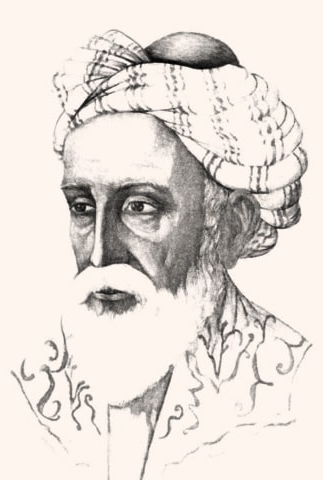
\includegraphics[height=0.5\textheight]{images/omar_khayyam.png}
\end{center}


\clearpage
\renewcommand{\rightmark}{Задания}
Выполняя каждое задание, используйте систему контроля версий \git{}. Следите за~оформлением кода, выбирайте подходящие имена переменным и функциям. Тщательно готовьте тесты (тестовые сценарии игры, вычисления). Не~перекладывайте работу разработчика на~плечи проверяющего. Это поможет и вам самим убедиться в~работоспособности кода после внесённых изменений. Задавайте вопросы на~семинарах.

\textbf{NB!} Данные задания "--- это только повод для~беседы. В~процессе сдачи могут быть заданы дополнительные вопросы и подзадачи.



%%=====================
\subsection{Задание №1}
%%=====================
%%=====================
\subparagraph{Часть 1.}
%%=====================
\textit{Игра <<Ним>>}

\bigskip\noindent
\begin{minipage}[T]{0.58\columnwidth}\parindent=2.5em
    \emph{Ним} "--- одна из~самых старых и увлекательных математических игр. Для игры в~\emph{ним} необходим партнёр (в~\emph{ним} играют вдвоём), стол и набор фишек. В~качестве фишек обычно используются камешки или монетки. В~наиболее известном варианте \emph{нима} 12~фишек раскладываются в~три ряда так, как показано на~рисунке.

    Правила \emph{нима} просты. Игроки по~очереди забирают одну или несколько фишек из~любого ряда. Не~разрешается за~один ход брать фишки из~нескольких рядов. Выигрывает тот, кто возьмёт последнюю фишку (фишки).

    \smallskip

    Если вы сыграете несколько партий в~\emph{ним}, то скоро заметите, что существует некоторая оптимальная последовательность ходов, которая гарантирует победу, если только вы начинаете игру и первым ходом берёте две фишки из~первого ряда. Любой другой ход даст шанс вашему сопернику, который в~этом случае наверняка победит, если, в~свою очередь, воспользуется оптимальной стратегией.

    Полный анализ игры с~обобщением на~любое число рядов с~любым числом фишек в~каждом ряду впервые опубликовал в~1901~г. профессор математики из~Гарвардского университета Чарльз Л.\,Бутон (\textenglish{Charles L.\,Bouton}), который и назвал игру «ним» от~устаревшей формы английских глаголов «стянуть», «украсть».
\end{minipage}\hfill\begin{minipage}[T]{0.4\columnwidth}
    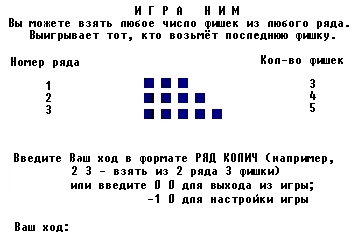
\includegraphics[width=\columnwidth]{images/nim_start_game.jpg}
\end{minipage}

\bigskip

\textbf{Разработайте программу}, которая будет выполнять роль партнёра в~игре, причём это будет весьма опасный противник, так как он будет «знать» оптимальную стратегию и умело ею пользоваться.

\medskip

\textbf{Срок сдачи}: не~позднее \deadline{30~сентября}.



%%=====================
\subparagraph{Часть 2.}
%%=====================
\textit{Калькулятор}

Доработайте окончательную версию калькулятора из~\textbookref{главы~7} учебника Бьярне Страуструпа, выполнив упражнения с~1-го по~9-е включительно.

Используйте <<тестовую оснастку>> для~автоматического тестирования программы. Для~этого подготовьте файл с~входными выражениями, как верными, так и ошибочными. Подавайте содержимое этого файла на~вход калькулятора, а~его вывод направьте в~другой файл. Проверьте выходные данные и запомните под~иным именем. При~повторном запуске программы после внесения изменений сравнивайте [программно] новый полученный файл с~проверенными ответами. Количество тестовых примеров для~финальной версии должно превышать~50.

Сгруппируйте исходный код логически, поместив каждую часть (функции, классы, их методы, константы) в~отдельный файл и связав её с~другими частями при~помощи заголовочного файла. Используйте идеи \textbookref{главы~8}.

\medskip

\textbf{Срок сдачи}: не~позднее \deadline{14~октября}.



%%==================================
\subsection{Контрольная работа №\,1}
%%==================================
%%==========================================
\subparagraph{Требования к оформлению кода:}
%%==========================================
\ldots



\vspace{0pt plus 2fil}
%%=======================
\subsection{Задание №\,2}
%%=======================
%%=====================
\subparagraph{Часть 1.}
%%=====================
\textit{Элементы графики}

Разработайте версию простой логической игры или некоторой полезной программы с~использованием элементов графики и графического пользовательского интерфейса на~основе библиотек \name{Graph\_lib} и \name{FLTK}.

Опишите кратко (тезисно) этапы создания программы: анализ задачи, идеи, какие классы в~каком порядке создавались и редактировались, с~какими сложностями сталкивались в~процессе проектирования/реализации. Оформите эти записи в~\href{https://ru.wikipedia.org/wiki/Markdown}{\lang{Markdown}} или в~простом текстовом файле. Можно использовать ключевые фрагменты кода.

\smallskip

\emph{Ограничение}: программа должна быть без~анимации.

\medskip

\textbf{Срок сдачи}: не~позднее \deadline{2~декабря}.


%%=====================
\subparagraph{Часть 2.}
%%=====================
\textit{Реализация вектора}

Запрограммируйте финальную версию вектора по~материалам \textbookref{главы~19} учебника Бьярне Страуструпа.

Напишите тестовый код, демонстрирующий работоспособность всего функционала. Используйте класс \code{Tracer} из~семинаров, если сочтёте необходимым.

\medskip

\textbf{Срок сдачи}: не~позднее \deadline{16~декабря}.



%%==================================
\subsection{Контрольная работа №\,2}
%%==================================
Основной нитью через всю контрольную проходит работа с~указателями и памятью непосредственно. Во~всех задачах будет включен контроль работы с~памятью, используя \code{valgrind}. То есть любые ошибки памяти, включая утечки, будут ошибками работы вашей программы.

%%==========================================
\subparagraph{Требования к оформлению кода:}
%%==========================================
такие же, как в~первой контрольной.



\newenvironment{results}[1][0pt]{
    \phantom{top of the page}
    \vspace{0pt plus 1fill}

    \noindent\hspace{#1}
    \begin{minipage}{\dimexpr\textwidth-#1\relax}
}{
    \end{minipage}

    \vspace{0pt plus 1fill}
    \phantom{bottom of the page}
}


\clearpage
\renewcommand{\rightmark}{Учебный план}
\begin{results}
    \input{data/curricula}
\end{results}


\clearpage
\renewcommand{\rightmark}{}
\begin{pycode}
import parse
import pathlib

import google_serve as gs


parse.set_rubicon(0.6)
datadir = pathlib.Path("data")
gc = gs.get_sheet(datadir/"token.json")
tabs = parse.read_json(datadir/"google_sheet.json")
for url in tabs["urls"]:
    title, table = parse.read_table(gc, url)
    print(rf"\groupsection{{{title}}}")
    print(rf"\renewcommand{{\rightmark}}{{\groupmark{{{title}}}}}")
    print("")
    print(r"\begin{results}")
    parse.print_main(table)
    print(r"\end{results}")
    print("")
    print(r"\clearpage")
    print(r"\begin{results}%[-0.5em]")
    parse.print_quiz(table)
    print(r"\end{results}")
    print("\n\n\n")
    print(r"\clearpage")
\end{pycode}

\end{document}
